% \documentclass[12pt,handout,xcolor=pdftex,dvipsnames,table]{beamer} %For handouts.
\documentclass[pdf]{beamer}
%\usepackage{pgfpages} %For handouts.
% This is the file main.tex
% \usepackage{handoutWithNotes}
\usepackage{subcaption} % subfigure
\usepackage{hyperref}
\usepackage{graphicx}
\usepackage[en-US]{datetime2} % fix warning of \author[*]{\today}
\usepackage{lmodern}% http://ctan.org/pkg/lm (For special Fonts)
\usepackage{ragged2e} % justify document
\usepackage{tikz}
\usepackage{smartdiagram}
\usepackage{xcolor}
% \usepackage{subfig}
\usepackage{multicol}

\mode<presentation>
\setbeamertemplate{blocks}[rounded][shadow=true]
\usetheme{Dresden} % so so
\setbeamertemplate{page number in head/foot}[totalframenumber]
\setbeamertemplate{navigation symbols}{} %take out the navigation symbols
\setbeamertemplate{caption}[numbered] %enumerate the caption and tables
\usefonttheme[stillsansseriflarge]{structureitalicserif}
  
%\mode<handout>{\setbeamercolor{background canvas}{bg=black!5}} %For handouts.
% \pgfpagesuselayout{4 on 1 with notes}[a4paper,border shrink=5mm]
  
%\makeatletter %reset the numbering on the subfigures (1)
%\@addtoreset{subfigure}{figure} %reset the numbering on the subfigures (2)
%\makeatother %reset the numbering on the subfigures (3)

%For Large figures
%\includegraphics[width=\linewidth,height=\textheight,keepaspectratio]{SMS}

\title{Azure Replicable CI / CD Locally} % (optional, only for long titles)
\subtitle{
	\href{https://github.com/thanos1983/beamerAzureCiCdLocal}
    		{GitHub Project Repo: beamerAzureCiCdLocal}
}
\author[Athanasios Garyfalos]{Author: Athanasios Garyfalos \\*
Date: \today } % (optional, for multiple authors)
% {A.~Garyfalos \and A.~Garyfalos2 \and A.~Garyfalos3}
\institute[garyfalos@cpan.org] % (optional)
{
	\\
	\medskip
	{
	% \emph{A.atga12@student.bth.se}
	% \emph{Another Author email}
	% \emph{Another Author}
	}
}
% \vspace*{-0.5cm}
% \date{Date: \today} % Multi page content
% \subject{Sample of Work Demonstration Django Rest Framework}

% \AtBeginSection[]{
%  \begin{frame}
%    \frametitle{Table of Contents}
%    \tableofcontents[currentsection]
%  \end{frame}
% }

\AtBeginSubsection[]{
  \begin{frame}<beamer>
    \begin{multicols}{2}
      \tableofcontents[currentsection,hideothersubsections]
    \end{multicols}
  \end{frame}
}

\begin{document}
	\begin{frame}[noframenumbering]
  \begin{center}
    % Upper part of the page
    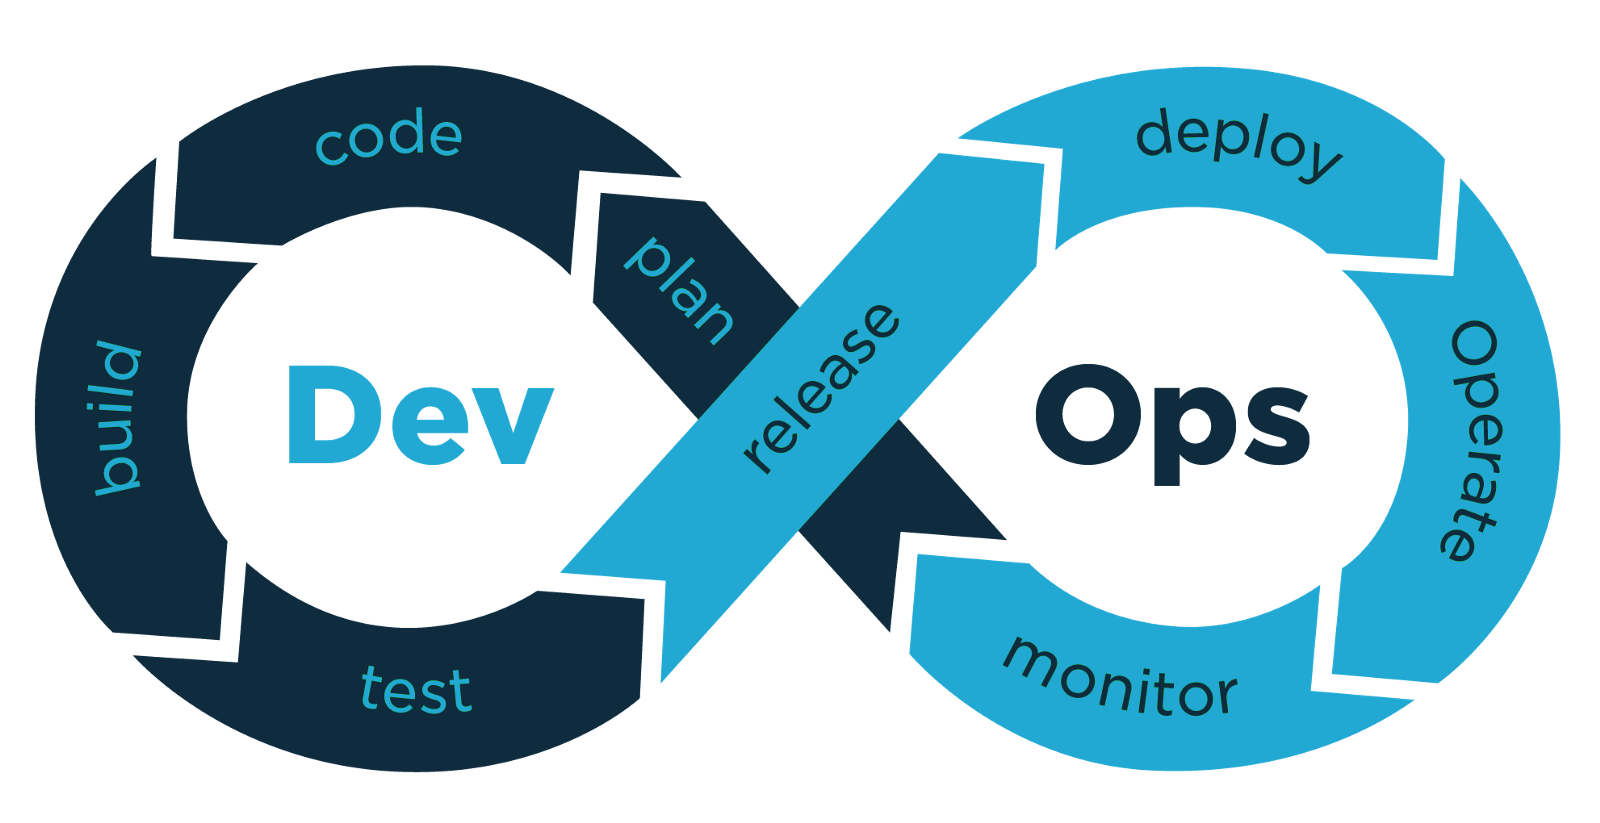
\includegraphics[width=.5\textwidth]{png/devopsAzure}\\ % [0.3cm]
  \end{center}
  \titlepage
\end{frame}

	% \section*{Copyright Disclaimer}
  \begin{frame}
    \begin{justify}
      {\justifying Copyright \alert{Disclaimer}: This program is free software: you can redistribute it and/or modify it under the terms of the GNU General Public License as published by the Free Software Foundation, either version 3 of the License, or (at your option) any later version.
      \bigbreak
      This program is distributed in the hope that it will be useful, but WITHOUT ANY WARRANTY; without even the implied warranty of MERCHANTABILITY or FITNESS FOR A PARTICULAR PURPOSE.  See the GNU General Public License for more details.
      \bigbreak
      You should have received a copy of the GNU General Public License along with this program.  If not, see.~\cite{gnuLicences} }
    \end{justify}
\end{frame}

	\section*{Contents}
% \begin{frame}[allowframebreaks]{Outline} % Multi page content
%  \setbeamercovered{dynamic} % Makes the text appear before it presents nice!!!
%  \tableofcontents[pausesections, sections={1-4}]
%    \framebreak
%  \tableofcontents[pausesections, sections={4-8}]
% \end{frame}
\begin{frame}
  \setbeamercovered{dynamic} % Makes the text appear before it presents nice!!!
  \begin{multicols}{2}
    \tableofcontents
  \end{multicols}
\end{frame}

	\section{Introduction} \label{sec:funtamentals}
\subsection{Why to Replicate CI / CD Locally}

\begin{frame}{High level description of the problem}
\setbeamercovered{dynamic}%Makes the text appear before it presents nice!!!!
	\begin{columns}[T] % contents are top vertically aligned
		\begin{column}{5cm} % each column can also be its own environment
			\begin{itemize}
				\item<+-| alert@+> It works locally why not remotely?
				\item<+-| alert@+> It works on my computer why not on yours?
				\item<+-| alert@+> Common Wrong Assumptions:
					\begin{itemize}
						\item<+-| alert@+> Running same package(s) version
						\item<+-| alert@+> No difference on installation process
						\item<+-| alert@+> No difference between Operating Systems
					\end{itemize}
				\item<+-| alert@+> Is there a solution?
			\end{itemize}
		\end{column}
		\begin{column}{5cm} % alternative top-align that's better for graphics
			\begin{figure}
				\only<1>{%
					\centering Local Vs Remote
					
\includegraphics[width=\columnwidth, height=0.5\textheight]{./png/personThinking}
				}%
				\only<2>{%
					\centering Not replicable
					
\includegraphics[width=\columnwidth, height=0.5\textheight]{./png/worksOnLocal}
				}%
				\only<3>{%
					\centering Wrong Assumptions
					
\includegraphics[width=\columnwidth, height=0.5\textheight]{./png/presume}
				}%
				\only<4>{%
					\centering Major / Minor Version
					
\includegraphics[width=\columnwidth, height=0.5\textheight]{./png/majorMinor}
				}%
				\only<5>{%
					\centering Is there a difference in compilers?
					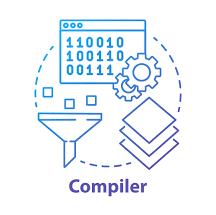
\includegraphics[width=\columnwidth, height=0.5\textheight]{./png/compiler}
				}%
				\only<6>{%
					\centering Windows vs Mac vs Linux
					
\includegraphics[width=\columnwidth, height=0.5\textheight]{./png/windowsMacLinux}
				}%
				\only<7>{%
					\centering Maybe...
					
\includegraphics[width=\columnwidth, height=0.5\textheight]{./png/letsSee}
				}%
				\caption{Problem Overview} \label{fig:largeFigure}
			\end{figure}
		\end{column}
	\end{columns}
\end{frame}

	\section{Software Development} \label{sec:cicd}
\subsection{Overall Problems}

\begin{frame}{Cross OS Programming Languages}
\setbeamercovered{dynamic}%Makes the text appear before it presents nice!!!!
	\begin{columns}[T] % contents are top vertically aligned
		\begin{column}{5cm} % alternative top-align that's better for graphics
		\begin{figure}
			\only<1>{%
				\centering Python
				
\includegraphics[width=\columnwidth, height=0.5\textheight]{./png/python}
			}%
			\only<2>{%
				\centering Python2 Deprecated
				
\includegraphics[width=\columnwidth, height=0.5\textheight]{./png/python2}
			}%
			\only<3>{%
				\centering Python3 Active
				
\includegraphics[width=\columnwidth, height=0.5\textheight]{./png/python3}
			}%
			\only<4>{%
				\centering Node JS
				
\includegraphics[width=\columnwidth, height=0.5\textheight]{./png/nodeJs}
			}%
			\only<5>{%
				\centering Under Development
				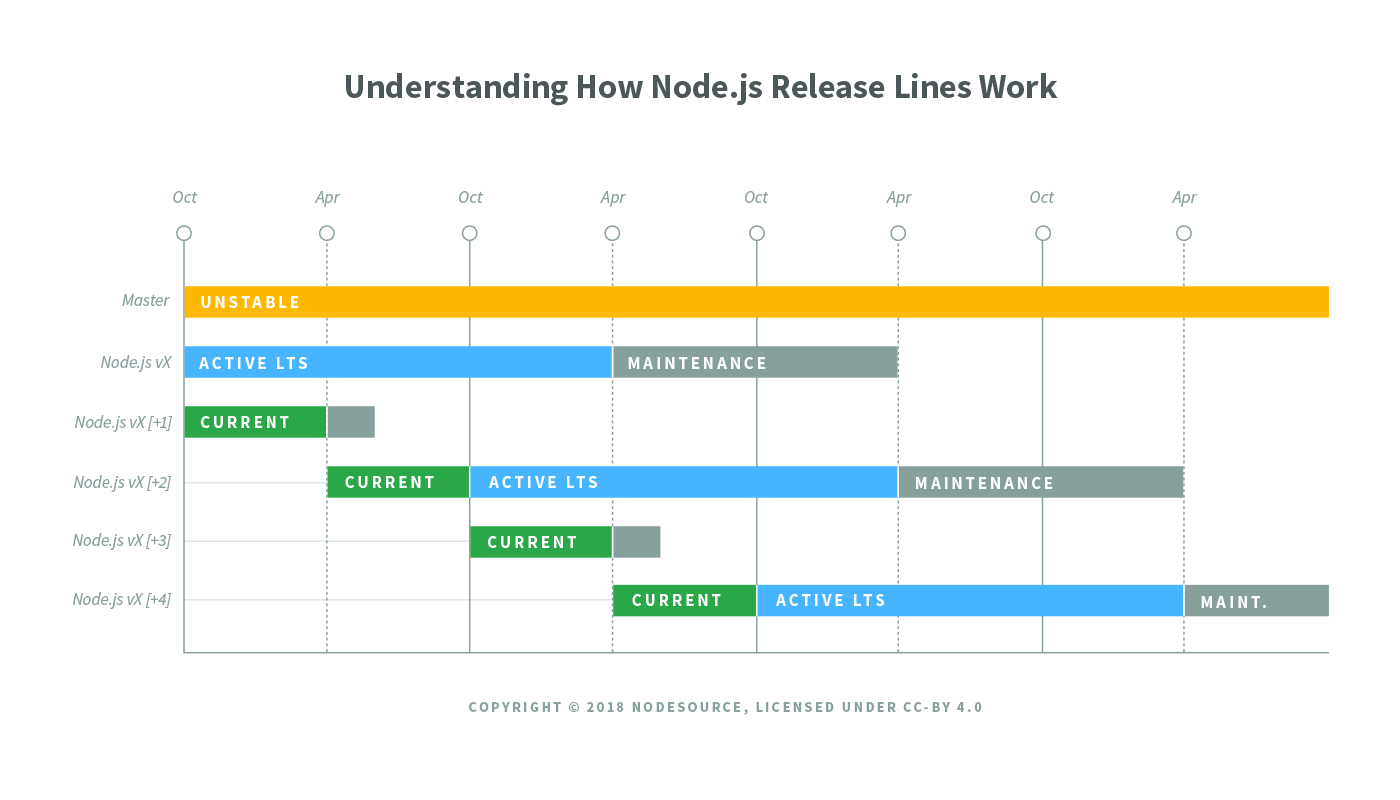
\includegraphics[width=\columnwidth, height=0.5\textheight]{./png/nodejsRelease}
			}%
			\only<6>{%
				\centering Current Latest Release
				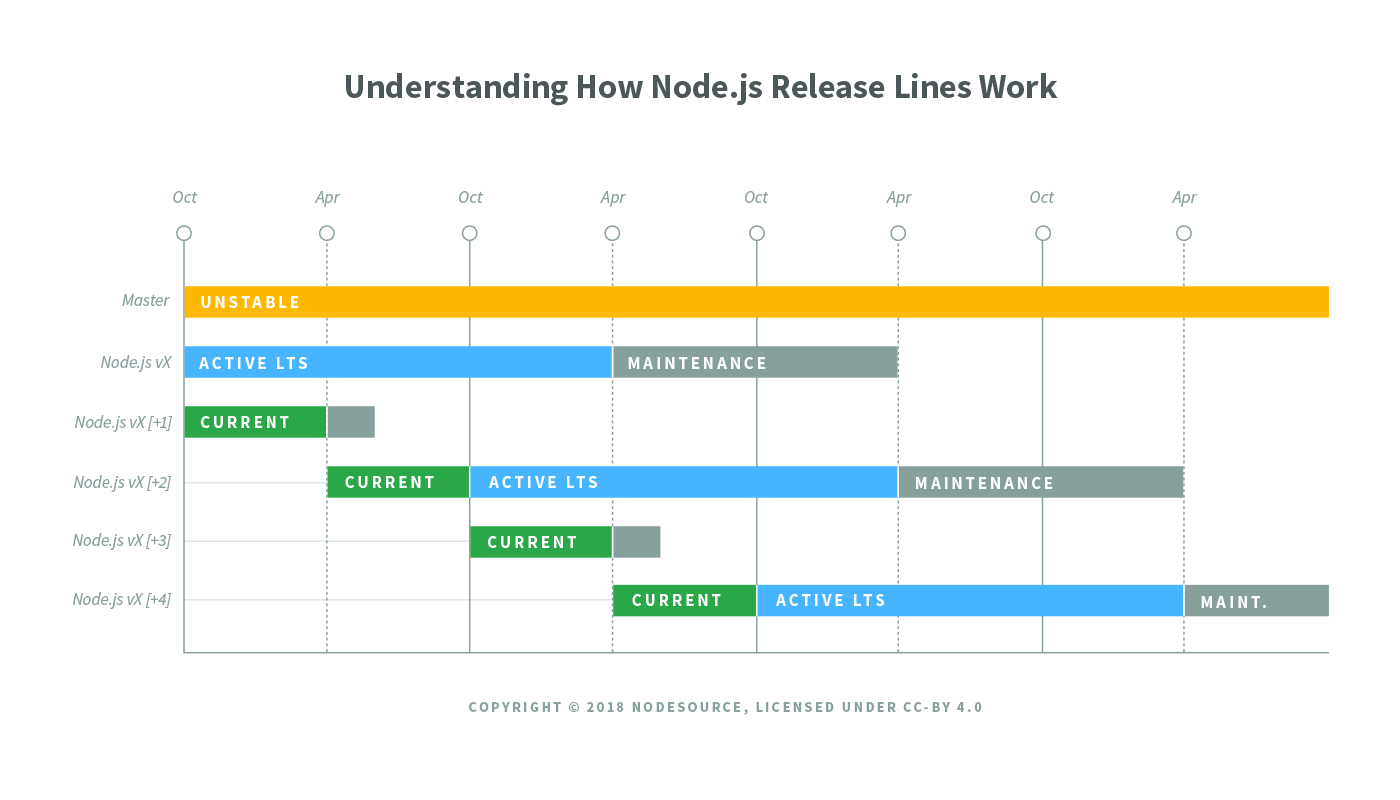
\includegraphics[width=\columnwidth, height=0.5\textheight]{./png/nodejsRelease}
			}%
			\only<7>{%
				\centering Active Long Term Support
				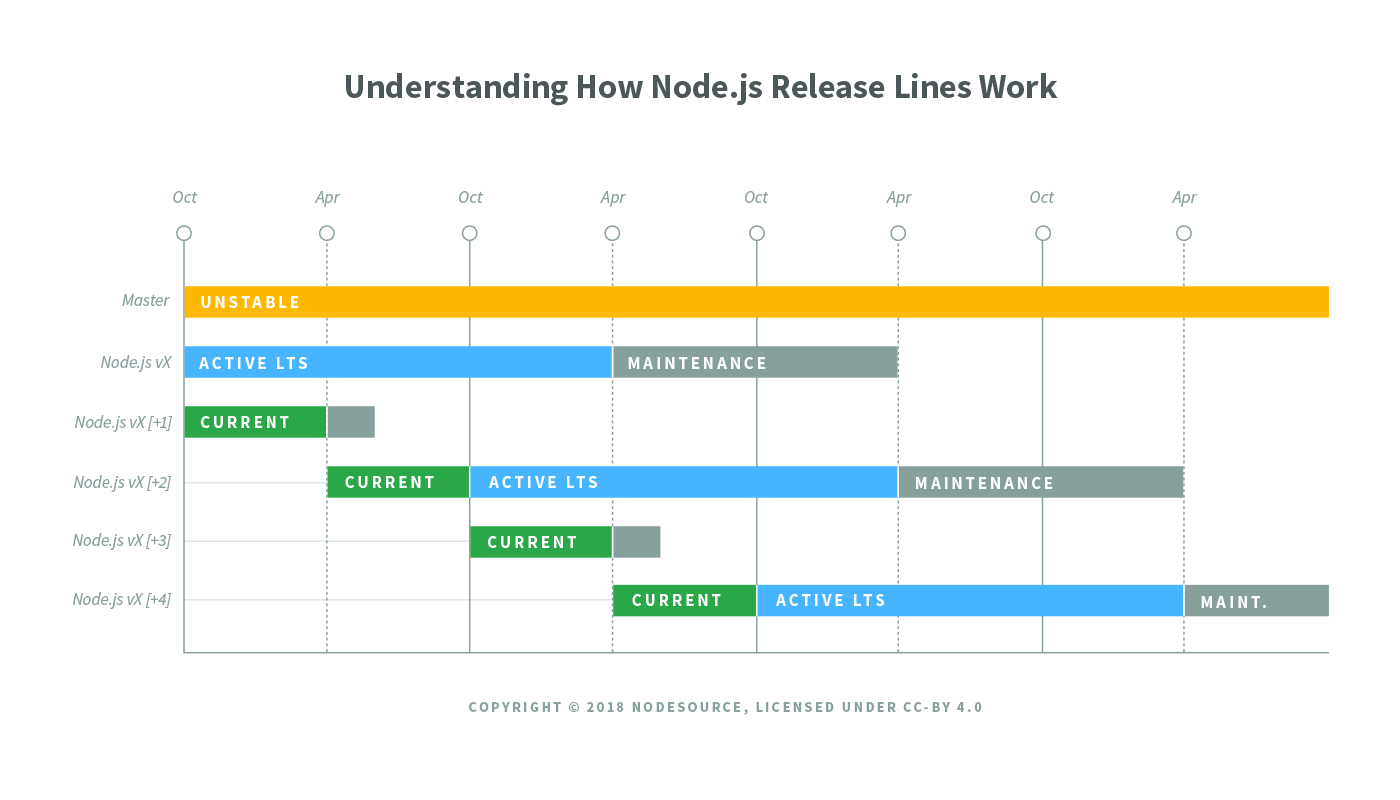
\includegraphics[width=\columnwidth, height=0.5\textheight]{./png/nodejsRelease}
			}%
			\only<8>{%
				\centering Maintenance Long Term Support
				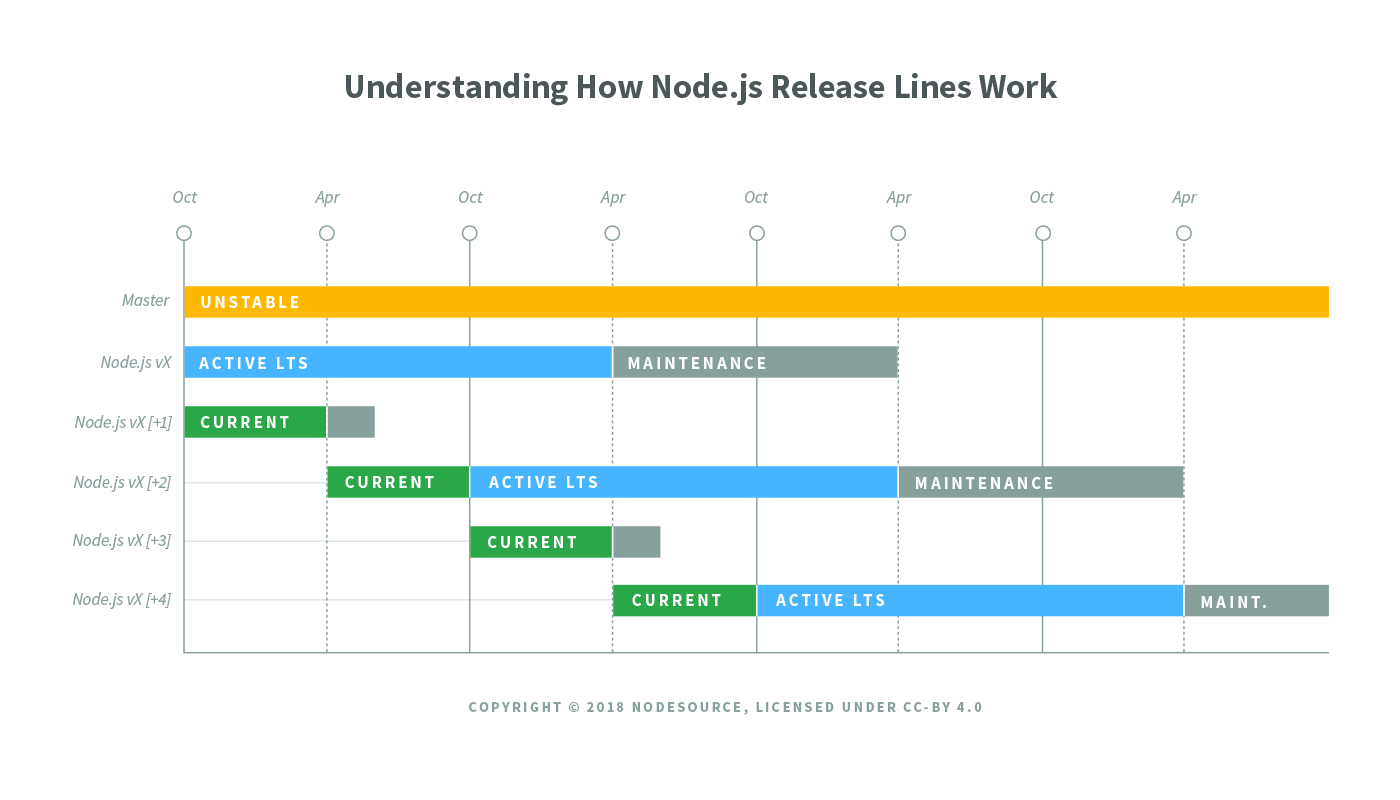
\includegraphics[width=\columnwidth, height=0.5\textheight]{./png/nodejsRelease}
			}%
			\only<9>{%
				\centering Tons of versions
				
\includegraphics[width=\columnwidth, height=0.5\textheight]{./png/java}
			}%
			\only<10>{%
				\centering Java Oracle
				
\includegraphics[width=\columnwidth, height=0.5\textheight]{./png/javaOracle}
			}%
			\only<11>{%
				\centering Java OpenJDK
				
\includegraphics[width=\columnwidth, height=0.5\textheight]{./png/openjdk}
			}%
			\only<12>{%
				\centering Maintenance Long Term Support (LTS)
				
\includegraphics[width=\columnwidth, height=0.5\textheight]{./png/AdoptOpenJDK}
			}%
			\only<13>{%
				\centering Different Installation Process
				
\includegraphics[width=\columnwidth, height=0.5\textheight]{./png/packageInstaller}
			}%
			\only<14>{%
				\centering Bundle package
				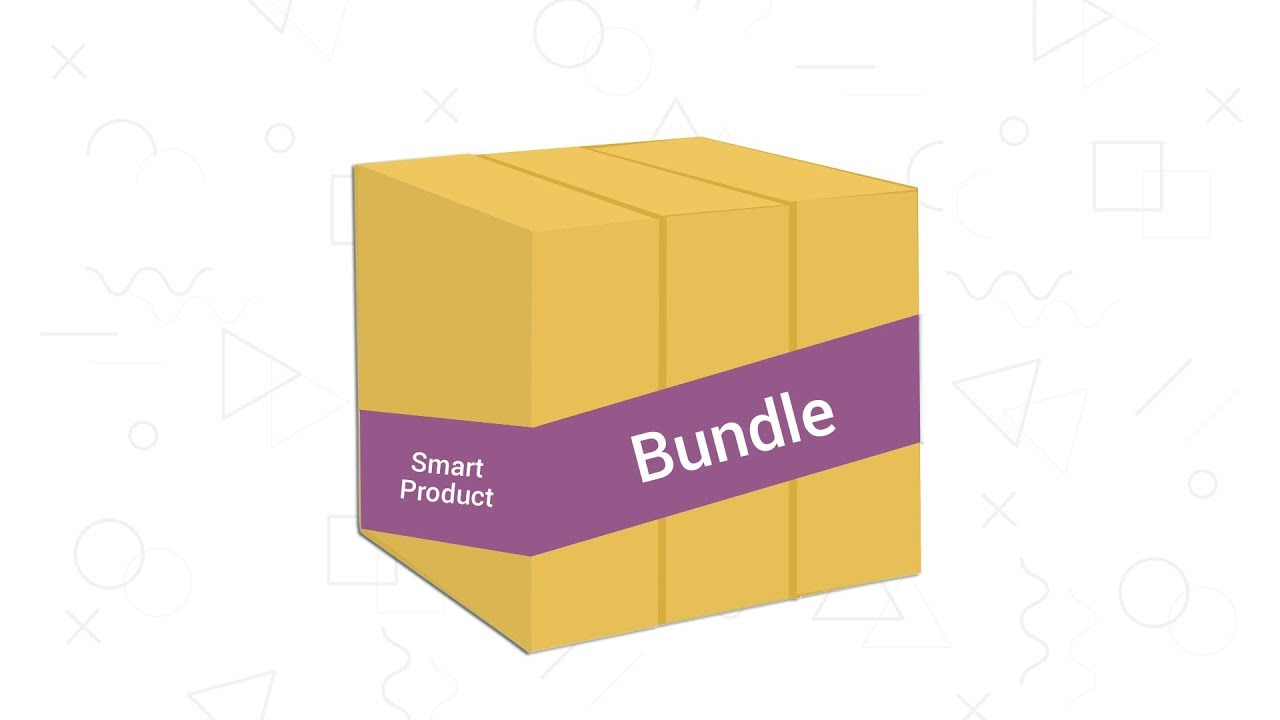
\includegraphics[width=\columnwidth, height=0.5\textheight]{./png/bundle}
			}%
			\only<15>{%
				\centering Source Code
				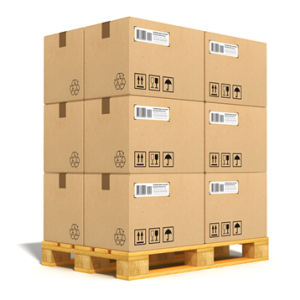
\includegraphics[width=\columnwidth, height=0.5\textheight]{./png/packageBySource}
			}%
			\caption{Problem Overview} \label{fig:smallFigure}
		\end{figure}
		\end{column}
		\begin{column}{5cm} % each column can also be its own environment
			\begin{itemize}
				\item<+-| alert@+> Python:
					\begin{itemize}
						\item<+-| alert@+> Python2
						\item<+-| alert@+> Python3
					\end{itemize}
				\item<+-| alert@+> Node.js
					\begin{itemize}
						\item<+-| alert@+> Pending
						\item<+-| alert@+> Current
						\item<+-| alert@+> Active LTS
						\item<+-| alert@+> Maintenance LTS
					\end{itemize}
				\item<+-| alert@+> Java:
					\begin{itemize}
						\item<+-| alert@+> Oracle
						\item<+-| alert@+> OpenJDK
						\item<+-| alert@+> AdoptOpenJDK
					\end{itemize}
				\item<+-| alert@+> Cross Platform OS
			\end{itemize}
		\end{column}
	\end{columns}
\end{frame}

\subsection{Simple Solution}

\begin{frame}{Impossible vs Possible}
	\setbeamercovered{dynamic} %Makes the text appear before it presents nice!!!!
	\begin{alertblock}{Impossible Solution}
		\begin{itemize}
			\item<+-| alert@+> Everyone needs to have exactly same \alert{OS}.
			\item<+-| alert@+> Everyone needs to install packages \alert{the same way}.
			\item<+-| alert@+> Everyone must update the OS and package \alert{at the same time}.
			\item<+-| alert@+> To what extent this is \alert{possible and practical}?
		\end{itemize}
	\end{alertblock}
	\begin{figure}
		\only<5>{%
			\centering Containers again and again
			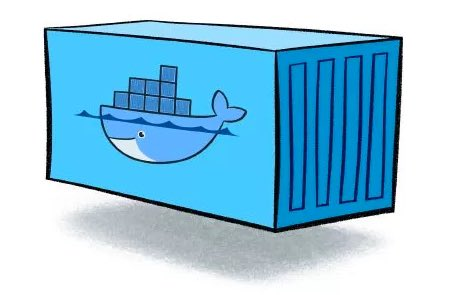
\includegraphics[width=\columnwidth, height=0.5\textheight]{./png/dockerContainer}
		}%
	\end{figure}
\end{frame}
	\section{Implementation} \label{sec:implementation}
\subsection{CI-CD Local}

\begin{frame}{Local Procedure}
\setbeamercovered{dynamic}%Makes the text appear before it presents nice!!!!
	\begin{columns}[T] % contents are top vertically aligned
		\begin{column}{5cm} % each column can also be its own environment
			\resizebox{5cm}{!}{%
				\smartdiagramset{set color list={blue!40!yellow,
										blue!40!orange,
										blue!40!red,
										blue!40!purple,
										blue!40!gray
										},
				}
				\tikzset{priority arrow/.append style={rotate=180,
											anchor=0,
											xshift=30
											}
				}
				\smartdiagram[priority descriptive diagram]{Stop Clean up,
													Deploy with volumes / ports - Validation tests,
													Build / Push Image - Cleanup volumes / networks,
													Login Docker Registry - Vault (https) with encrypted credentials,
													Prepare Dockerfile with parameters
												}
			}%
		\end{column}
		\begin{column}{5cm} % alternative top-align that's better for graphics
			\begin{itemize}
				\item<+-| alert@+> Dockerfile (template).
				\item<+-| alert@+> Vault (https).
				\item<+-| alert@+> Any socket.
					\begin{itemize}
						\item<+-| alert@+> Azzure Registry.
						\item<+-| alert@+> Build Dockerfile.
						\item<+-| alert@+> Push Image.
						\item<+-| alert@+> Logout Azzure.
						\item<+-| alert@+> Prune everything.
						\item<+-| alert@+> Raise error (if).
					\end{itemize}
				\item<+-| alert@+> Deployment (volume).
				\item<+-| alert@+> Validation (tests).
				\item<+-| alert@+> Stop, Cleanup.
			\end{itemize}
		\end{column}
	\end{columns}
\end{frame}

\subsection{CI-CD Kubernetes}

\begin{frame}{Local k8s Deployment Procedure}
\setbeamercovered{dynamic}%Makes the text appear before it presents nice!!!!
	\begin{columns}[T] % contents are top vertically aligned
		\begin{column}{5cm} % each column can also be its own environment
			\resizebox{5cm}{!}{%
				\smartdiagramset{set color list={blue!40!yellow,
										blue!40!orange,
										blue!40!red,
										blue!40!purple
										},
				}
				\tikzset{priority arrow/.append style={rotate=180,
											anchor=0,
											xshift=30
											}
				}
				\smartdiagram[priority descriptive diagram]{Stop Clean up / Roll Back,
													Validation tests,
													Pull Image / Deploy with volumes / services etc ,
													Login Docker Registry - Vault (https) with encrypted credentials
												}
			}%
		\end{column}
		\begin{column}{5cm} % alternative top-align that's better for graphics
			\begin{itemize}
				\item<+-| alert@+> Vault (https).
				\item<+-| alert@+> Any socket.
					\begin{itemize}
						\item<+-| alert@+> Azzure Registry.
						\item<+-| alert@+> Pull Image.
					\end{itemize}
				\item<+-| alert@+> Deployment (volume).
				\item<+-| alert@+> Logout Azzure.
				\item<+-| alert@+> Validation (tests).
					\begin{itemize}
						\item<+-| alert@+>Raise error (if).
						\item<+-| alert@+> Stop, Cleanup.
						\item<+-| alert@+> Roll back.
					\end{itemize}
			\end{itemize}
		\end{column}
	\end{columns}
\end{frame}

% \begin{frame}
%  \centering
%  \begin{figure}
%    \only<1-3>{
%        \begin{subfigure}[b]{0.3\textwidth}
%          \caption{Free Positioning}
%                \includegraphics[width=\textwidth,height=\textwidth]{./png/crio}
%                \label{fig:guided}
%                \setcounter{subfigure}{0}% Reset subfigure counter
%        \end{subfigure}\hfill
%        }
%    \only<2-3>{
%        ~ %add desired spacing between images, e. g. ~, \quad, \qquad etc.
%          %(or a blank line to force the subfigure onto a new line)
%        \begin{subfigure}[b]{0.3\textwidth}
%        \setcounter{subfigure}{1}% Reset subfigure counter
%          \caption{Neural Network}
%                \includegraphics[width=\textwidth,height=\textwidth]{./png/cri}
%                \label{fig:free}
%        \setcounter{subfigure}{0}% Reset subfigure counter
%        \end{subfigure}\hfill
%        }
%    \only<3-3>{
%        ~ %add desired spacing between images, e. g. ~, \quad, \qquad etc.
%          %(or a blank line to force the subfigure onto a new line)
%        \begin{subfigure}[b]{0.3\textwidth}
%            \setcounter{subfigure}{2}% Reset subfigure counter
%          \caption{Matlab Output}
%                \includegraphics[width=\textwidth,height=\textwidth]{./png/pod}
%                \label{fig:multiple}
%        \end{subfigure}%
%        }
%        \caption{Different wireless charging approaches~\label{fig:animals}}
%  \end{figure}
%  \begin{itemize}[<+->]
%      \item<1-| alert@1> Free positioning charging based on Inductive coupling~\cite{wireless}.
%      \item<2-| alert@2> Based on RLoad and Frequency Input and Output~\cite{wireless}. %\ref{fig:free}
%      \item<3-| alert@3> Simulation of Matlab Output based on RLoad as an Input~\cite{wireless}. %   \ref{fig:multiple}
%  \end{itemize} 
%\end{frame}

	\section{Demo}
\subsection{Demo CI / CD}

\begin{frame}
\setbeamercovered{dynamic}
	\begin{center}
		\Huge \textcolor{cyan}{\emph{Coming up: Demo}}
	\end{center}
\end{frame}
	\section{Summary}
\subsection{Key points repetition}

\begin{frame}
\setbeamercovered{dynamic}
	\begin{exampleblock}{Summary}
		\begin{itemize}[<+->]
			\item In section~``\nameref{sec:funtamentals}'' page ``\ref{sec:funtamentals}'' Common issues, non replicable.
			\item In section~``\nameref{sec:cicd}'' page ``\ref{sec:cicd}'' Variety of programming languages and the problems.
			\item In section~``\nameref{sec:implementation}'' page ``\ref{sec:implementation}'' CI / CD Flow Build / Deploy / Test. \pause
		\end{itemize}
	\end{exampleblock}
	\begin{exampleblock}{Extra Notes}
		\begin{itemize}[<+->]
			\item Demo on CI / CD build / deploy / validation and error handling cases.
			\item Both the CI / CD and Kubernetes project are provided as open source contribution. The Presentation was written in \alert{\LaTeX}
		\end{itemize}
	\end{exampleblock}
\end{frame}

\subsection*{Questions}
\begin{frame}
%\begin{overlayarea}{\textwidth}{3cm}
    %\only<1>{Some text for the first slide.\\Possibly several lines long.}
    %\only<2>{Replacement on the second slide.}
%\end{overlayarea}
	\begin{center}
		\Huge \textcolor{cyan}{\emph{Coming up: Q \& A}}
	\end{center}
\end{frame}
	\section{Bibliography}
\subsection*{Web and Articles}

\begin{frame}[allowframebreaks]
	\frametitle<presentation>{References}
	\bibliographystyle{amsalpha}
		\begin{thebibliography}{10}
		%\setbeamertemplate{bibliography item}[online]
		\setbeamertemplate{bibliography item}{
\includegraphics[width=1.5em]{./png/gnu}}
			\bibitem{gnuLicences}
				GNU LESSER GENERAL PUBLIC LICENSE
				\newblock {\emph{GNU Operating System}}
				\newblock available at \url{https://www.gnu.org/licenses/lgpl.html}.
		% \setbeamertemplate{bibliography item}[online]
		% \setbeamertemplate{bibliography item}{\includegraphics[width=1.5em]{./png/KubernetesRef}}
		%	\bibitem{KubernetesCri}
		%		Author: K.~Community
		%		\newblock {\emph{Container Runtimes}}
		%		\newblock available at \url{https://kubernetes.io/docs/setup/production-environment/container-runtimes/}.
		% \setbeamertemplate{bibliography item}[article]
		% \setbeamertemplate{bibliography item}{\includegraphics[width=1.3em]{./png/KubernetesRef}}
		%	\bibitem{kubernetesNetworking}
		%		Author: K.~Community
		%		\newblock {\emph{Cluster Networking}}
		%		\newblock available at \url{https://kubernetes.io/docs/concepts/cluster-administration/networking/}.
	\end{thebibliography}
\end{frame}
\end{document}
